\documentclass[tikz,border=5pt]{standalone}
\usepackage{pgfplots}
\pgfplotsset{compat=1.18}
\usepgfplotslibrary{fillbetween}

\begin{document}
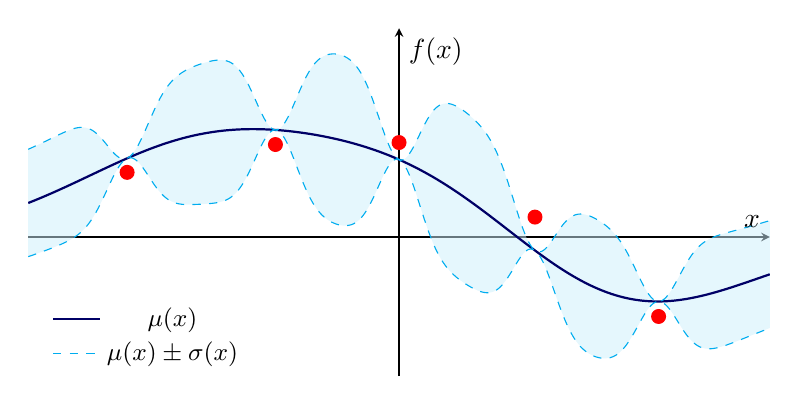
\begin{tikzpicture}
  \begin{axis}[
      width=11cm,
      height=6cm,
      axis lines=middle,
      xlabel={$x$},
      ylabel={$f(x)$},
      xmin=-3, xmax=3,
      ymin=-1.4, ymax=2.1,
      xtick=\empty,
      ytick=\empty,
      domain=-3:3,
      samples=400,
      legend style={at={(0.02,-0.)},anchor=south west,draw=none,fill=none,font=\small},
    ]

    % ---- 观测点位置（用于“藕节”） ----
    % x = -2.2, -1.0, 0.0, 1.1, 2.1

    % Posterior mean μ(x) – 示意函数
    \addplot[name path=mu, blue!40!black, thick]
    { 0.9*exp(-0.5*(x+1.6)^2)
      + 0.7*exp(-0.5*(x-0.2)^2)
      - 0.8*exp(-0.5*(x-1.8)^2)
    };
    \addlegendentry{$\mu(x)$}

    % 构造一个“在样本点为 0，远离样本点变大的” σ(x)
    % base(x): 整体验证度大小的轮廓
    % node factors: 在每个观测点附近压成 0
    \addplot[
      name path=upper,
      samples=400,
      cyan,
      dashed
    ]
    {
      % mean
      0.9*exp(-0.5*(x+1.6)^2)
      + 0.7*exp(-0.5*(x-0.2)^2)
      - 0.8*exp(-0.5*(x-1.8)^2)
      % + sigma(x)
      + (0.5 + 0.4*exp(-0.5*(x/1.4)^2))
        * (1 - exp(-18*(x + 2.2)^2))
        * (1 - exp(-18*(x + 1.0)^2))
        * (1 - exp(-18*(x - 0.0)^2))
        * (1 - exp(-18*(x - 1.1)^2))
        * (1 - exp(-18*(x - 2.1)^2))
    };

    \addplot[
      name path=lower,
      dashed,
      cyan,
      samples=400,
    ]
    {
      % mean
      0.9*exp(-0.5*(x+1.6)^2)
      + 0.7*exp(-0.5*(x-0.2)^2)
      - 0.8*exp(-0.5*(x-1.8)^2)
      % - sigma(x)
      - (0.5 + 0.4*exp(-0.5*(x/1.4)^2))
        * (1 - exp(-18*(x + 2.2)^2))
        * (1 - exp(-18*(x + 1.0)^2))
        * (1 - exp(-18*(x - 0.0)^2))
        * (1 - exp(-18*(x - 1.1)^2))
        * (1 - exp(-18*(x - 2.1)^2))
    };

    % 填充 μ ± σ 区间（藕状带）
    \addplot[
      fill=cyan!20,
      opacity=0.5
    ]
    fill between[
      of=upper and lower,
    ];
    \addlegendentry{$\mu(x)\pm\sigma(x)$}

    % 观测点
    \addplot[
      only marks,
      mark=*,
      mark size=2.5pt,
      color=red
    ]
    coordinates {
      (-2.2, 0.65)
      (-1.0,  0.93)
      ( 0.0,  0.95)
      ( 1.1,  0.20)
      ( 2.1, -0.80)
    };
    % \addlegendentry{observations}

  \end{axis}
\end{tikzpicture}
\end{document}